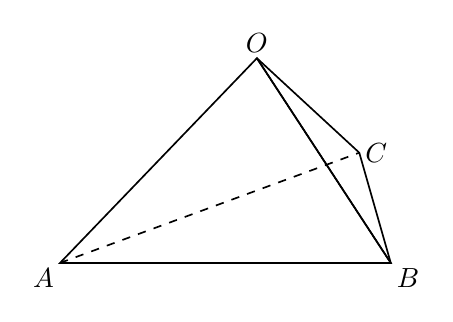
\begin{tikzpicture}[x=1cm,y=1cm,font=\normalsize,
  geometry edge/.style={solid,line width=.6pt},
  geometry label/.style={font=\normalsize,inner sep=2pt}]
\coordinate (O) at (2.5,3.2);
\coordinate (A) at (0,0.6);
\coordinate (B) at (4.2,0.6);
\coordinate (C) at (3.8,2.0);
\draw[geometry edge] (O)--(A)--(B)--cycle;
\draw[geometry edge] (O)--(B);
\draw[geometry edge] (O)--(C)--(B);
\draw[geometry edge,dashed] (A)--(C);
\node[geometry label,above] at (O) {$O$};
\node[geometry label,below left] at (A) {$A$};
\node[geometry label,below right] at (B) {$B$};
\node[geometry label,right] at (C) {$C$};
\end{tikzpicture}
